\section{Introduction to implementation}
This report explains our implementation of the project. \\
Overall the project uses the classes seen in Figure \ref{fig:UMLClassDiagram}

\begin{figure}[h!]
\centering
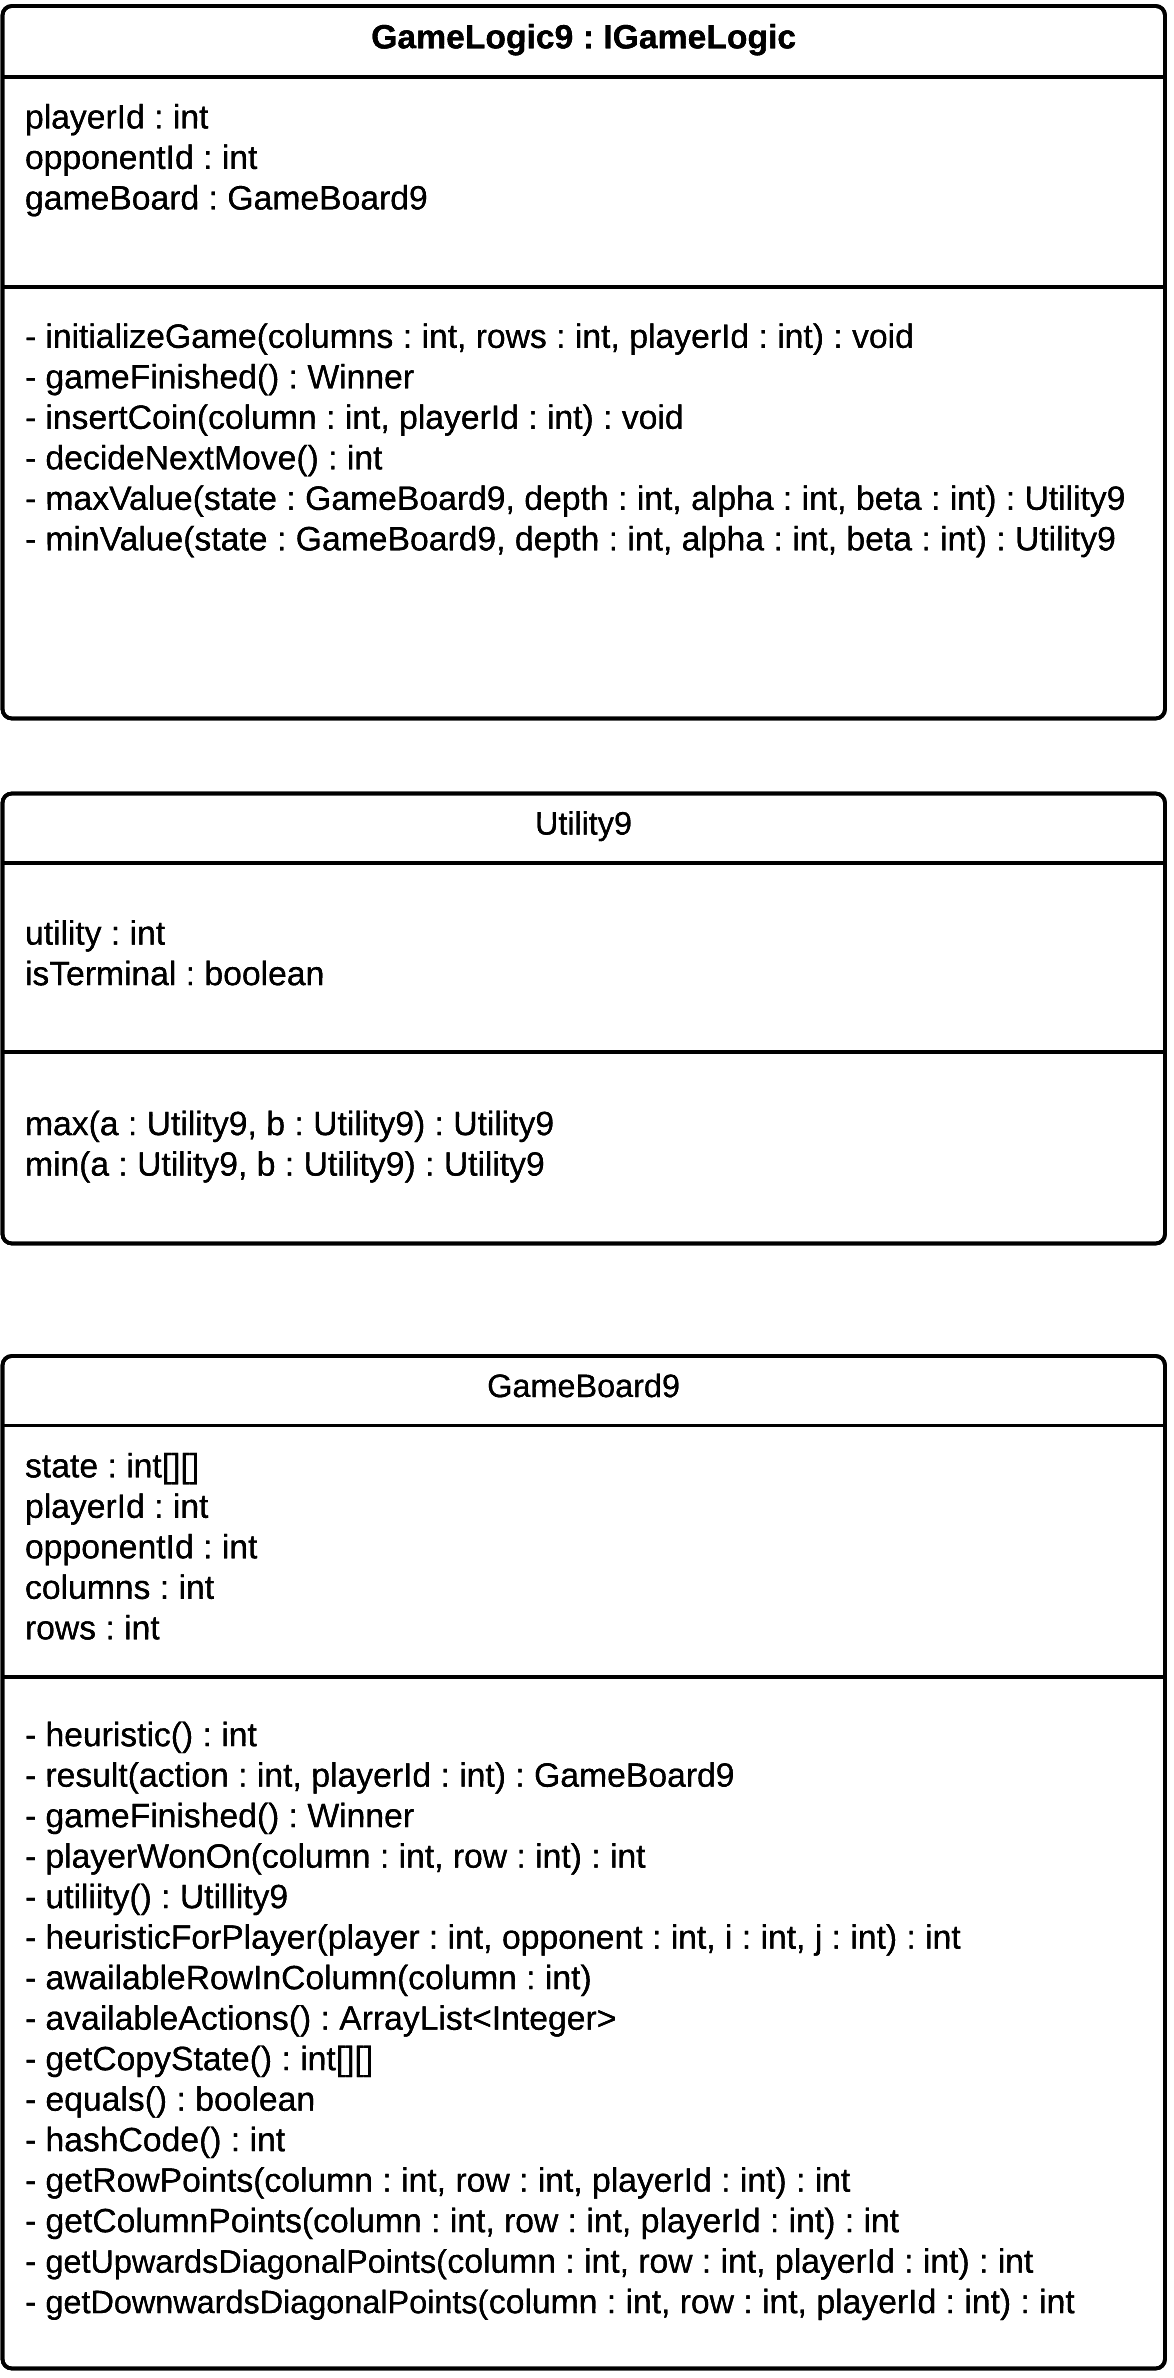
\includegraphics[width=0.65\linewidth]{ClassDiagram.png}
\caption{UML class-diagram showing off classes implemented by group \label{fig:UMLClassDiagram}}
\end{figure}

The class \texttt{Utility9} is used to represent utility. The functions \texttt{maxValue} and \texttt{minValue} returns \texttt{Utility9} instances. It has two fields; \texttt{utiliity} to represent some utility, and a flag, \texttt{isTerminal} stating whether this is a terminal state or not. \\
Moreover, \texttt{Utility9} provides two static methods, \texttt{max(...)} and \texttt{min(...)}, that takes as arguments two \texttt{Utility9} instances, and returns the largest and the smallest, respectively; determined by comparing their utility-values. 

The \texttt{Gameboard9} class is used to encapsulate logic in relation to (the state of) and operations on the gameboard. To name a few, this includes a utility-function, a result-function and a function that returns the available actions.

Because the \texttt{GameBoard9} is used as the key in a cache for utility values, the class also overrides the \texttt{hashCode}-function and the equals function. These only compares the actual game board state, which internally is represented as a 2D array of integers.

\subsection{Evaluation and cut-off function}



\subsection{$\alpha$-$\beta$ pruning}
The \texttt{GameLogic9} class implements an $\alpha-\beta$ pruning search algorithm. The idea is to reduce the search space, to only look at values that aren't already guaranteed to be matched, for either of min-value and max-value.